\RequirePackage{fix-cm}
%
%\documentclass{svjour3}                     % onecolumn (standard format)
\documentclass[smallcondensed]{svjour3}     % onecolumn (ditto)
%\documentclass[smallextended]{svjour3}       % onecolumn (second format)
%\documentclass[twocolumn]{svjour3}          % twocolumn
%
\smartqed  % flush right qed marks, e.g. at end of proof
%
%
\makeatletter
%\def\cl@chapter{\cl@chapter \@elt {theorem}}%bug in class
\def\cl@chapter{\@elt {theorem}}
\makeatother
%
\usepackage{times}  % DO NOT CHANGE THIS
\usepackage{helvet} % DO NOT CHANGE THIS
\usepackage{courier}  % DO NOT CHANGE THIS
\usepackage[hyphens]{url}  % DO NOT CHANGE THIS
\usepackage{graphicx} % DO NOT CHANGE THIS
\urlstyle{rm} % DO NOT CHANGE THIS
\def\UrlFont{\rm}  % DO NOT CHANGE THIS
\frenchspacing  % DO NOT CHANGE THIS
\setlength{\pdfpagewidth}{8.5in}  % DO NOT CHANGE THIS
\setlength{\pdfpageheight}{11in}  % DO NOT CHANGE THIS

\usepackage{latexsym}
\usepackage{amsmath}
\usepackage{amssymb}
\usepackage{subcaption}
\captionsetup{compatibility=false}
%\usepackage{caption}
\usepackage{cleveref}
\usepackage[normalem]{ulem}
\usepackage{array}
\usepackage{multirow}
\usepackage{booktabs} % For formal tables

\begin{document}

%\section{Appendix}
\section{Section 3.1.3 : Similarity by Contrast}
The exact view construction algorithm for similarity by contrast views are:

\textbf{TrueSkill Similarity} connects answers authored by a specific user, where the difference in his skill over peers is greater than margin $\delta$. Specifically, if the user authors answers $a, a'$ to questions $q, q'$, we create a link between $a$ and $a'$ if %$\lvert S_{u,a} - S_{u, b} \rvert > \delta; \forall b \in \mathcal{A}_(q)$ and $\lvert S_{u,a'} - S_{u, c} \rvert > \delta; \forall c \in \mathcal{A}_(q')$
\begin{align*}
 \lvert S_{u,a} - S_{u, b} \rvert &> \delta; \forall b \in \mathcal{A}_(q) \\
 \lvert S_{u,a'} - S_{u, c} \rvert &> \delta; \forall c \in \mathcal{A}_(q')
\end{align*}
where $S_{u,a}$ is the skill value for the user who authored answer $a$. Similarly, a link is created for the opposite case when difference is less than $-\delta$.
% \begin{align*}
% \lvert S_{u,a} - S_{u, b} \rvert < -\delta; \forall b \in \mathcal{A}(q) \\
% \lvert S_{u,a'} - S_{u, c} \rvert < -\delta; \forall c \in \mathcal{A}(q')
% \end{align*}

We estimate the user skill values with the TrueSkill rating system (\url{https://pypi.org/project/trueskill/}) computed with their historic performance in the community. TrueSkill values are normally distributed among users (\cref{fig:clique}).

% developed by Microsoft Reasearch for ranking and matching similar skill game players for Xbox Live. In our settings, each question is a multi player game with all answerers as game players. The user who gives credible answer is the winner. True Skill rating then computes player's skill through bayesian inference on the basis of credibility label of his answered questions. The estimated ratings are a Gaussian distribution where $\mu$ denotes the average skill of the player. We use the mean value as skill value for our computations.


\begin{figure}[th]
  \centering
  \begin{subfigure}{0.5\textwidth}
    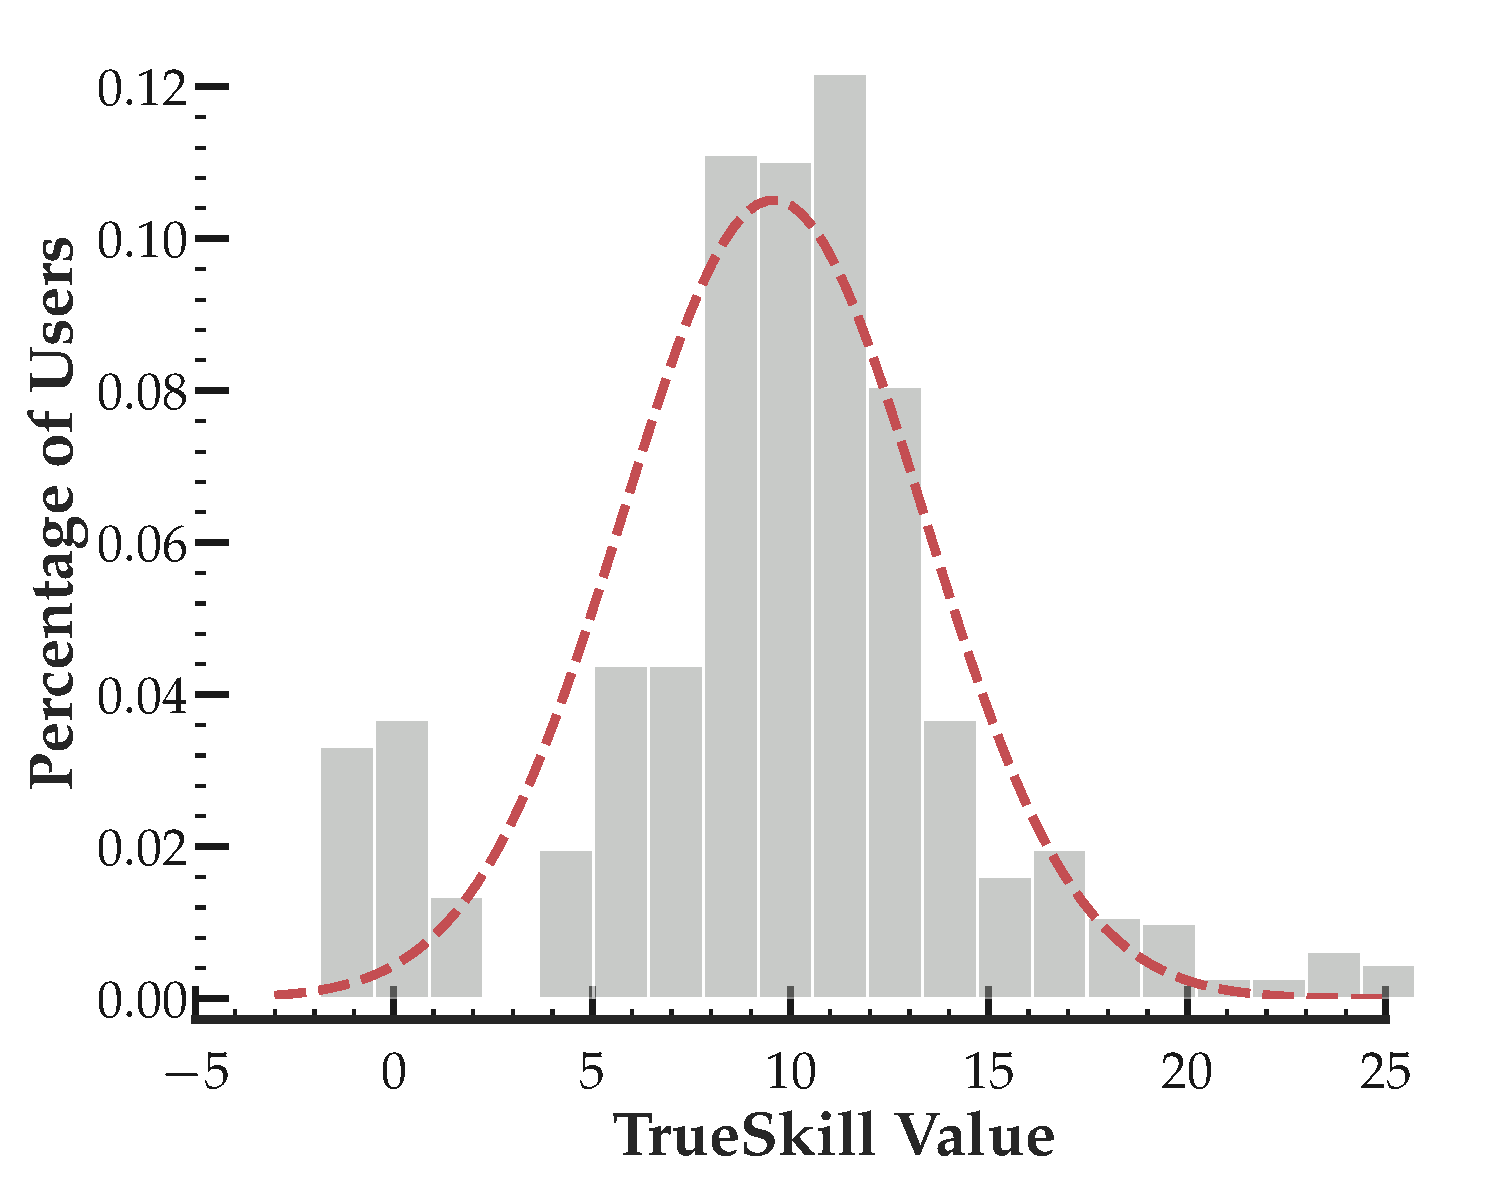
\includegraphics[scale=0.25]{figures/TrueSkill}
    \caption{TrueSkill Distribution}
  \end{subfigure}%
  \begin{subfigure}{0.5\textwidth}
    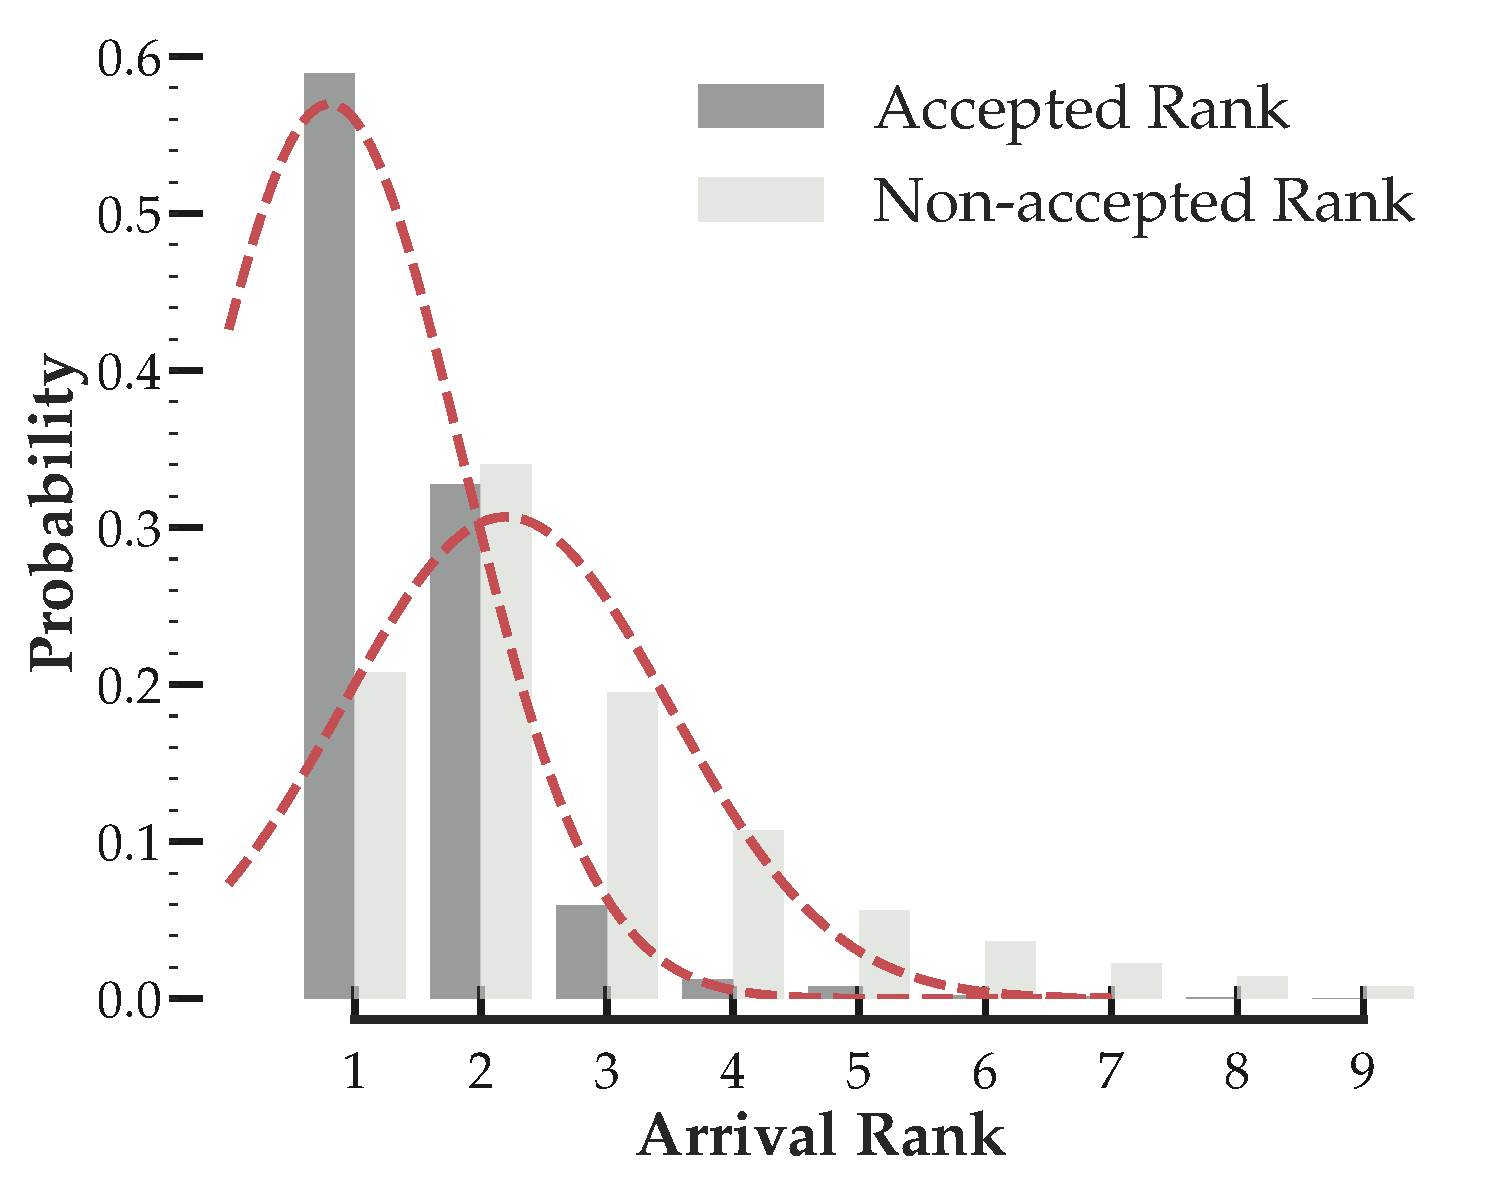
\includegraphics[scale=0.25]{figures/ArrivalRank}
    \caption{ArrivalRank Distribution}
  \end{subfigure}
  \caption{\label{fig:clique} Distribution of the TrueSkill values of users and ArrivalRank of accepted answers and non-accepted answers for the movie StackExchange. Early answers are more likely to be accepted and variance of TrueSkill similarity across users is high.}
\end{figure}

\textbf{Arrival Similarity}
The temporal arrival patterns of answers are correlated to their acceptance probabilities (\cref{fig:clique}). For a specific user authoring answers $a, a'$ to questions $q, q'$, we establish a link between these answers if %$\lvert T_{a} - T_{b} \rvert > \gamma \times \max(T_{b}); \forall b \in \mathcal{A}_(q)$ and $\lvert T_{a'} - T_{c} \rvert > \gamma \times \max(T_{c}); \forall c \in \mathcal{A}_(q')$.
%Highly skilled/active users tend to follow consistent patterns in when they author answers, relative to the other competing answers.
%We observe that earlier posted answers have a higher chance of acceptance in CQA platform as shown in Figure \ref{fig:clique}. Therefore,
\begin{align*}
 \lvert T_{a} - T_{b} \rvert &> \gamma \times \max(T_{b}); \forall b \in \mathcal{A}_(q) \\
 \lvert T_{a'} - T_{c} \rvert &> \gamma \times \max(T_{c}); \forall c \in \mathcal{A}_(q')
\end{align*}
where $T_{a}$ represents the relative time-gap between answer $a$ and the question $q$. Conversely, we create links when difference is less than $-\gamma \times \max(T_{b})$.
%\begin{align*}
% \lvert T_{a} - T_{b} \rvert < -\gamma * max(T_{b}); \forall b \in \mathcal{A}(q) \\
% \lvert T_{a'} - T_{c} \rvert < -\gamma * max(T_{c}); \forall c \in \mathcal{A}(q')
%\end{align*}
Our hypotheis is that a similar answering schedule indicates similar user confidence or skill across questions.

\section{Section 4.2 : Contrastive Convolution}
\label{ref:analysis}
In this section, we provide a theoretical analysis of our contrastive convolution.
The ability of neural networks to perform classification in sparse high-dimensional manifolds has been studied in past work, especially in the context of adversarial learning \cite{lu2017safetynet}. We employ the ReLU activation function in our convolution layers and study the outputs of the $k$th layer, i.e. embeddings with k-order locality. This transformation breaks the input space into cells with smooth gradients within each cell, at whose boundaries the piecewise linear function changes (i.e. the likelihood of the two classes of answers).

% In the context of adversarial learning \cite{safetynet} propose the existence of p-domains or cells in the learned manifold, representing a piecewise linear mapping of the transformed features to the class labels. The generalization neutrality property is particularly interesting. Both train and test samples are highly unlikely to lie in p-domains since the number of examples is much smaller than the capacity of the neural network to fit these regions. Weight decay can incentivize relatively small changes in the gradient across these regions resulting in smoother changes.  the ability of the network to fit such regions in the data manifold?

We ask a specific question in the context of our Contrastive IR-GCN. \emph{What is the impact of the layerwise discriminative magnification induced by our formulation?} Discriminative magnifications results in improved separability of the two classes in the later convolving layers, an effect we earlier demonstrated with a sample network in \cref{fig:contrast}. This positively impacts the ability of the model to explain the observed data points (i.e create p-domains that are well aligned with the contrastive samples provided) and improve the generalizability of the learned model to unseen data points. However, it is important to maintain sufficient regularization with weight decay to prevent sparse regions exhibiting sharp gradients which could affect model performance.

The capacity of our model can also be quantified in terms of the VC dimension of the aggregated classifier against the individual learners. Gradient boosting with multiple relation learners (each of which captures a specific aspect of node locality via graph convolution on the induced relations) could boost the capacity of the joint model, enabling better generalization and a more accurate fit in the data manifold (i.e. higher capacity to fit regions to fine distinctions).

Let us denote the upper bound of the VC dimension or capacity of each individual learner as D (If the individual learners do not have identical capacity, the minimum can be used to compute a lower bound on the aggregated learner capacity). Then the gradient boosted learner with T classifiers has a bound on it's capacity~\cite{shalev2014understanding} given by,
\begin{equation*}
\mathcal{VC}_{Agg}  = T \times (D+1) \times(3 \log(T.(D+1))+2)
\label{vcdim}
\vspace{-0.03in}
\end{equation*}

Thus we identify two potential reasons for our performance gains, first the discriminative magnification effect which also supports the strong individual performance of the contrast view, and second the gain in capacity from boosting, which could explain it's advantage over competing aggregation methods.

\section{Section 5 : Aggregating Induced Views}
The prior aggregation methods used in the literature were adapted for our GCN model as follows:

\textbf{Neighborhood Aggregation:} is a multi relational approach that aggregates neighbors of the nodes from all views. Thus, the final adjacency matrix is the sum of all the individual adjacency matrices of each view, i.e., $A = \sum_{S_i \in \mathbf{S}} A_i$. We, then, apply Graph Convolution Network to this updated Adjacency matrix.

\textbf{Stacking:} stacks all GCNs belonging to a view such that output of a lower GCN is fed as an input to the GCN directly above it. Thus, output from the last layer of GCN for view $i$, $Z_i^K$ s.t. $  S_i \in \textbf{S}$ will act as input features, $Z_j^0$ for some other view $j$ s.t. $S_j \in \{\textbf{S}-S_i \}$ if view $j$ is directly above the view $i$. In our experiments, we obtain the best performance by using the following order: Contrastive, Similarity by Contrast followed by Reflexive.

\textbf{Fusion:} treats each GCN as a separate model and appends the output from the final layer of each GCN i.e. $Z_i^K; \forall S_i \in \textbf{S}$ to the input of all the other GCN's, i.e. $Z_j^0 \forall S_j \in \textbf{S}-S_i$ along with the original features. Thus, the input of each GCN is linear in $\vert \textbf{S} \vert$.

\section{Section 6.1 : Dataset}
The list of 50 StackExchange communities per category are;
\begin{itemize}
\item Technology: AskUbuntu, Server Fault, Unix, TEX, Electronics, Gis, Apple, Wordpress, Drupal, DBA

\item Culture/Recreation: English, Travel, RPG, Judaism, Puzzling, Bicycles, German, Christianity, BoardGames, History

\item Life/Arts: Scifi, DIY, Academia, Graphic Design, Money, Photo, WorldBuilding, Movies, Music, Law

\item Science: Stat, Physics, MathOverflow, CS, Chemistry, Biology, Philosophy, CS Theory, Economics, Astronomy

\item Professional/Business: Workplace, Aviation, Writers, Open source, Freelancing, CS Educators, Quant, PM, Parenting
\end{itemize}

\section{Section 6.2.1 : Baselines }
\textbf{Dual GCN (DGCN)} The mean squared error (MSE) between vertex representations of two views is defined as, for instance,
\begin{equation*}
 \mathcal L_{reg}(Z_c, Z_{ts}) = \frac{1}{n} \sum_{j \in {1,n}}  \lVert Z_c^j - Z_{ts}^j \lVert
\end{equation*}
computes the MSE loss between Contrastive and TrueSkill Similarity GCN.
\cite{DualGCN} proposed the model for two GCN representations.
We extend the original two GCN model \cite{DualGCN} to four GCN, each representing our relational views between the nodes. We minimize the supervised loss with respect to the best performing GCN model (Contrastive), and its node representation's alignment with respect to all other GCN's node representations.
The Contrastive view is seen to exhibit the best performance in isolation. Thus, the DualGCN loss can be given by:
\begin{equation*}
  %\mathcal L  = \mathcal L_0(Z_c) + \lambda{(t)} \left( \mathcal L_{reg}(Z_c, Z_{ts}) + \mathcal L_{reg}(Z_c, Z_{as}) + \mathcal L_{reg}(Z_c, Z_r) \right)
  \mathcal L  = \mathcal L_0 +  \lambda{(t)} \left( \sum_{S_i \in \mathbf{S}, S_i \neq c} \lVert \mathbf{Z}_c^K - \mathbf{Z}_i^K \lVert \right)
\end{equation*}
where $\mathcal L_0$ represents the supervised loss and $\mathbf{Z}_c^K$ is the node representations of the Contrastive GCN.

\noindent
\textbf{Relational GCN (RGCN)} \cite{relationalGCN} combines the output representations of previous layer of each view $\mathbf{Z}_i^{k-1}$ of layer $k-1$ of each view to compute an aggregated input to layer $k$.
Formally,
\begin{equation*}
  \mathbf{Z}_{rgcn}^{k} = \sigma \left( \sum_{S_i \in \mathbf{S}} \mathbf{Z}_i^{k-1}\right)
\end{equation*}
where $Z_{rgcn}$ is final output of this model at layer $k$ and $\sigma$ is the activation function.

\section{Section 6.3 : Performance Analysis}
The breakdown of the results by the StackExchange community are given in the tables below.(Technology: \cref{tab:stackacc}, Culture: \cref{tab:stackacc2}, Life: \cref{tab:stackacc3}, Science: \cref{tab:stackacc4}, Business: \cref{tab:stackacc5}).
\begin{table*}[h]
  %\robustify\bfseries
  %\small
  \centering
    %\setlength{\tabcolsep}{0.5pt}
 %\begin{tabular}{l|S[round-mode=places,round-precision=2]@{\hspace{1mm}}S@{\hspace{1mm}}|S[round-mode=places,round-precision=2]@{\hspace{1mm}}S@{\hspace{1mm}}|S[round-mode=places,round-precision=2]@{\hspace{1mm}}S@{\hspace{1mm}}|S[round-mode=places,round-precision=2]@{\hspace{1mm}}S@{\hspace{1mm}}|S[round-mode=places,round-precision=2]@{\hspace{1mm}}S@{\hspace{1mm}}S[round-mode=places,round-precision=2]@{\hspace{1mm}}S@{\hspace{1mm}}}
 %\begin{tabular}{l|S[round-mode=places,round-precision=2]S|S[round-mode=places,round-precision=2]S|S[round-mode=places,round-precision=2]S|S[round-mode=places,round-precision=2]S|S[round-mode=places,round-precision=2]SS[round-mode=places,round-precision=2]S}
 %\resizebox{1.5\columnwidth}{!}{
 \begin{subtable}{\textwidth}
  \begin{tabular}{l|c c|c c|c c|c c|c c}
     \toprule
     \multirow{2}{*}{Method} &
        \multicolumn{2}{c}{\textbf{AskUbuntu}} &
       \multicolumn{2}{c}{\textbf{Serverfault}} &
       \multicolumn{2}{c}{\textbf{Unix}} &
       \multicolumn{2}{c}{\textbf{TEX}} &
       \multicolumn{2}{c}{\textbf{Electronics}}\\
       &{Acc(\%)} & {MRR}&{Acc(\%)} & {MRR}&{Acc(\%)}& {MRR}&{Acc(\%)} & {MRR}&{Acc(\%)} & {MRR}\\
       %\cmidrule(lr){1-1}\cmidrule(lr){2-21}%\cmidrule(lr){12-21}
       \midrule
     \textbf{RF~\cite{BurelMA16,TianZL13}} & 64.63 & 0.668 & 68.38 & 0.648 & 70.90 & 0.597 & 64.93 & 0.717 & 67.69 & 0.699\\


     \textbf{FF~\cite{JendersKN16}} & 68.49 & 0.789 & 68.29 & 0.769 & 73.14 & 0.730 & 65.43 & 0.795 & 68.26 & 0.797\\
     %biLSTM & 63.84 & 0.6887 & 64.40 & 0.6772 & 70.65 & 0.5679 & 58.27 & 0.6944 & 58.10 & 0.6939 & 64.31 & 0.5869 \\
     %biLSTM+CNN & 67.86 & 0.7115 & 68.95 & 0.7009 & 73.08 & 0.6253 & 61.15 & 0.7050 & 59.15 & 0.7279 & 66.75 & 0.5997 \\
     \textbf{DGCN~\cite{DualGCN}} & 70.25 & 0.794 & 72.01 & 0.768 & 75.16 & 0.749 & 69.02 & 0.788 & 70.62 & 0.783 \\
     \textbf{RGCN~\cite{relationalGCN}} & 55.24 & 0.636 & 58.04 & 0.689 & 64.14 & 0.610 & 56.22 & 0.750 & 53.18 & 0.640\\
     \cmidrule(lr){1-1}\cmidrule(lr){2-11}%\cmidrule(lr){12-21}
     \textbf{AS-GCN} & 70.15 &0.774 & 68.09 & 0.751 &74.90 & 0.749 & 65.91 & 0.782 & 67.91 & 0.775 \\
     \textbf{TS-GCN} & 69.49 & 0.782 & 67.15 & 0.752 & 73.95 & 0.748 & 64.67 & 0.777 & 66.58 &0.777\\
     \textbf{C-GCN } & 72.27 & 0.792 & 72.42 & 0.772 & 76.44 & 0.761& 69.10 & 0.794 & 72.45 & 0.797\\
     %\textbf{IR-GCN} & \bfseries 73.96 $\pm$ \bfseries 0.023 & \bfseries0.7939\ \ \  $\pm$ \bfseries 0.014 & \bfseries 78.61 $\pm$ \bfseries 0.018 & \bfseries 0.7905 \ \ \ $\pm$ \bfseries 0.025 & \bfseries 79.21 $\pm$ \bfseries 0.032 & \bfseries 0.7995 \ \ \ $\pm$ \bfseries 0.037 & \bfseries 74.98 $\pm$ \bfseries 0.021 & \bfseries 0.8085 \ \ \ $\pm$ \bfseries0.028 & \bfseries80.17 $\pm$ \bfseries 0.026 & \bfseries 0.7849 \ \ \ $\pm$ \bfseries 0.032\\
     \textbf{IR-GCN} & \textbf{75.25} & \textbf{0.798} & \bfseries 73.87 & \bfseries 0.776 & \bfseries 78.75 & \bfseries 0.765 & \textbf{70.96} & \textbf{0.796} & \textbf{74.63} & \textbf{0.799} \\
     \bottomrule
   \end{tabular}\\
   \begin{tabular}{l|c c|c c|c c|c c|c c}
      \toprule
      \multirow{2}{*}{Method} &
         \multicolumn{2}{c}{\textbf{GIS}} &
        \multicolumn{2}{c}{\textbf{Apple}} &
        \multicolumn{2}{c}{\textbf{Wordpress}} &
        \multicolumn{2}{c}{\textbf{Drupal}} &
        \multicolumn{2}{c}{\textbf{DBA}}\\
        &{Acc(\%)} & {MRR}&{Acc(\%)} & {MRR}&{Acc(\%)}& {MRR}&{Acc(\%)} & {MRR}&{Acc(\%)} & {MRR}\\
        %\cmidrule(lr){1-1}\cmidrule(lr){2-21}%\cmidrule(lr){12-21}
        \midrule
      \textbf{RF~\cite{BurelMA16,TianZL13}} & 64.93 & 0.698 & 70.13 & 0.644 & 65.11 & 0.718 & 65.65 & 0.727 & 65.44 & 0.718\\


      \textbf{FF~\cite{JendersKN16}} & 64.69 & 0.786 & 68.86 & 0.785 & 64.62 & 0.805 & 64.88 & 0.799 & 66.39 & 0.803\\
      %biLSTM & 63.84 & 0.6887 & 64.40 & 0.6772 & 70.65 & 0.5679 & 58.27 & 0.6944 & 58.10 & 0.6939 & 64.31 & 0.5869 \\
      %biLSTM+CNN & 67.86 & 0.7115 & 68.95 & 0.7009 & 73.08 & 0.6253 & 61.15 & 0.7050 & 59.15 & 0.7279 & 66.75 & 0.5997 \\
      \textbf{DGCN~\cite{DualGCN}} & 68.51 & 0.775 & 73.52 & 0.770 & 70.11 & 0.808 & 68.22 & 0.791 & 69.58 & 0.793 \\
      \textbf{RGCN~\cite{relationalGCN}} & 50.30 & 0.671 & 49.48 & 0.627 & 55.89 & 0.729 & 51.26 & 0.688 & 50.30 & 0.686\\
      \cmidrule(lr){1-1}\cmidrule(lr){2-11}%\cmidrule(lr){12-21}
      \textbf{AS-GCN} & 64.82 & 0.771 & 69.76 & 0.776 & 65.00 & 0.791 & 65.06 & 0.785 & 65.95 & 0.793 \\
      \textbf{TS-GCN} & 64.13 & 0.799 & 68.94 & 0.773 & 63.80 & 0.795 & 64.41 & 0.786 & 65.55 & 0.797\\
      \textbf{C-GCN } & 69.12 & 0.787 & 73.08 & 0.785 & 70.80 & 0.809 & 70.69 & 0.802 & 69.99 & 0.818\\
      %\textbf{IR-GCN} & \bfseries 73.96 $\pm$ \bfseries 0.023 & \bfseries0.7939\ \ \  $\pm$ \bfseries 0.014 & \bfseries 78.61 $\pm$ \bfseries 0.018 & \bfseries 0.7905 \ \ \ $\pm$ \bfseries 0.025 & \bfseries 79.21 $\pm$ \bfseries 0.032 & \bfseries 0.7995 \ \ \ $\pm$ \bfseries 0.037 & \bfseries 74.98 $\pm$ \bfseries 0.021 & \bfseries 0.8085 \ \ \ $\pm$ \bfseries0.028 & \bfseries80.17 $\pm$ \bfseries 0.026 & \bfseries 0.7849 \ \ \ $\pm$ \bfseries 0.032\\
      \textbf{IR-GCN} & \textbf{71.20} & \textbf{0.791} & \bfseries 75.85 & \bfseries 0.791 & \bfseries 73.39 & \bfseries 0.814 & \textbf{73.43} & \textbf{0.802} & \textbf{72.25} & \textbf{0.806} \\
      \bottomrule
    \end{tabular}
    \end{subtable}
  %}
  \caption{\label{tab:stackacc} Accuracy and MRR values for StackExchange communities belonging to \textbf{Technology} category with state-of-the-art baselines.}
\end{table*}


\begin{table*}[h]
  %\robustify\bfseries
  %\small
  \centering
  \begin{tabular}{l|c c|c c|c c|c c|c c}
     \toprule
     \multirow{2}{*}{Method} &
        \multicolumn{2}{c}{\textbf{English}} &
       \multicolumn{2}{c}{\textbf{Travel}} &
       \multicolumn{2}{c}{\textbf{RPG}} &
       \multicolumn{2}{c}{\textbf{Judaism}} &
       \multicolumn{2}{c}{\textbf{Puzzling}}\\
       &{Acc(\%)} & {MRR}&{Acc(\%)} & {MRR}&{Acc(\%)}& {MRR}&{Acc(\%)} & {MRR}&{Acc(\%)} & {MRR}\\
       %\cmidrule(lr){1-1}\cmidrule(lr){2-21}%\cmidrule(lr){12-21}
       \midrule
         \textbf{RF~\cite{BurelMA16,TianZL13}}&73.98&0.564&70.94&0.655&73.29&0.590&70.16&0.665&73.94&0.548\\
          \textbf{FF~\cite{JendersKN16}}&73.36&0.755&73.70&0.802&72.92&0.765&67.96&0.780&73.90&0.738\\
          \textbf{DGCN~\cite{DualGCN}}&77.03&0.750&76.05&0.796&74.47&0.738&72.68&0.752&75.74&0.738\\
          \textbf{RGCN~\cite{relationalGCN}}&60.70&0.621&61.95&0.546&60.45&0.639&57.59&0.670&60.35&0.621\\
          \cmidrule(lr){1-1}\cmidrule(lr){2-11}
          \textbf{AS-GCN}&74.52&0.736&72.66&0.791&74.60&0.752&70.24&0.754&75.09&0.722\\
          \textbf{TS-GCN}&73.97&0.736&71.44&0.794&73.20&0.752&69.57&0.763&74.15&0.727\\
          \textbf{C-GCN}&76.67&0.752&76.49&0.802&77.07&0.767&73.31&0.783&77.47&0.745\\
          \textbf{IR-GCN}&\textbf{78.74}&\textbf{0.761}&\textbf{78.96}&\textbf{0.810}&\textbf{79.13}&\textbf{0.773}&\textbf{75.58}&\textbf{0.798}&\textbf{79.75}&\textbf{0.747}\\

     \bottomrule
   \end{tabular}\\
   \begin{tabular}{l|c c|c c|c c|c c|c c}
      \toprule
      \multirow{2}{*}{Method} &
         \multicolumn{2}{c}{\textbf{Bicycles}} &
        \multicolumn{2}{c}{\textbf{German}} &
        \multicolumn{2}{c}{\textbf{Christianity}} &
        \multicolumn{2}{c}{\textbf{BoardGames}} &
        \multicolumn{2}{c}{\textbf{History}}\\
        &{Acc(\%)} & {MRR}&{Acc(\%)} & {MRR}&{Acc(\%)}& {MRR}&{Acc(\%)} & {MRR}&{Acc(\%)} & {MRR}\\
        %\cmidrule(lr){1-1}\cmidrule(lr){2-21}%\cmidrule(lr){12-21}
        \midrule
        \textbf{RF~\cite{BurelMA16,TianZL13}}&74.09&0.604&69.85&0.675&74.67&0.607&71.49&0.677&72.83&0.683\\

        \textbf{FF~\cite{JendersKN16}}&73.86&0.789&69.56&0.781&72.26&0.791&72.01&0.814&72.69&0.806\\

        \textbf{DGCN~\cite{DualGCN}}&76.38&0.769&72.28&0.773&74.23&0.775&76.71&0.814&76.73&0.810\\

        \textbf{RGCN~\cite{relationalGCN}}&59.74&0.651&58.47&0.675&60.78&0.685&60.74&0.686&63.21&0.661\\
        \cmidrule(lr){1-1}\cmidrule(lr){2-11}
        \textbf{AS-GCN}&74.74&0.757&69.25&0.757&74.01&0.772&71.23&0.785&74.14&0.805\\

        \textbf{TS-GCN}&73.89&0.755&68.24&0.761&73.88&0.774&69.22&0.790&74.08&0.791\\

        \textbf{C-GCN}&77.79&0.773&73.02&0.779&76.63&0.786&76.43&0.816&76.90&0.815\\

        \textbf{IR-GCN}&\textbf{80.18}&\textbf{0.785}&\textbf{75.11}&\textbf{0.786}&\textbf{79.59}&\textbf{0.806}&\textbf{78.84}&\textbf{0.819}&\textbf{80.22}&\textbf{0.821}\\
      \bottomrule
    \end{tabular}
  %}
  \caption{\label{tab:stackacc2} Accuracy and MRR values for StackExchange communities belonging to \textbf{Culture} category with state-of-the-art baselines.}
\end{table*}

\begin{table*}[h]
  %\robustify\bfseries
  %\small
  \centering
  \begin{tabular}{l|c c|c c|c c|c c|c c}
     \toprule
     \multirow{2}{*}{Method} &
        \multicolumn{2}{c}{\textbf{SciFi}} &
       \multicolumn{2}{c}{\textbf{DIY}} &
       \multicolumn{2}{c}{\textbf{Academia}} &
       \multicolumn{2}{c}{\textbf{Graphic Design}} &
       \multicolumn{2}{c}{\textbf{Money}}\\
       &{Acc(\%)} & {MRR}&{Acc(\%)} & {MRR}&{Acc(\%)}& {MRR}&{Acc(\%)} & {MRR}&{Acc(\%)} & {MRR}\\
       %\cmidrule(lr){1-1}\cmidrule(lr){2-21}%\cmidrule(lr){12-21}
       \midrule
       \textbf{RF~\cite{BurelMA16,TianZL13}}&77.15&0.675&71.52&0.651&74.37&0.560&69.82&0.638&72.19&0.608\\

       \textbf{FF~\cite{JendersKN16}}&76.57&0.826&70.76&0.795&73.62&0.767&69.79&0.795&71.06&0.777\\

       \textbf{DGCN~\cite{DualGCN}}&79.27&0.818&74.67&0.794&76.92&0.757&74.43&0.792&74.80&0.770\\

       \textbf{RGCN~\cite{relationalGCN}}&59.56&0.651&58.08&0.690&64.36&0.672&59.11&0.712&60.58&0.652\\
      \cmidrule(lr){1-1}\cmidrule(lr){2-11}
       \textbf{AS-GCN}&74.67&0.816&70.18&0.778&75.26&0.732&70.01&0.784&72.19&0.755\\

       \textbf{TS-GCN}&61.13&0.793&69.40&0.788&74.20&0.740&69.17&0.782&70.98&0.751\\

       \textbf{C-GCN}&79.77&0.824&74.68&0.798&77.75&0.759&74.51&0.800&75.18&0.771\\

       \textbf{IR-GCN}&\textbf{81.60}&\textbf{0.834}&\textbf{76.83}&\textbf{0.805}&\textbf{79.62}&\textbf{0.772}&\textbf{76.13}&\textbf{0.804}&\textbf{77.11}&\textbf{0.784}\\
     \bottomrule
   \end{tabular}\\
   \begin{tabular}{l|c c|c c|c c|c c|c c}
      \toprule
      \multirow{2}{*}{Method} &
         \multicolumn{2}{c}{\textbf{Photo}} &
        \multicolumn{2}{c}{\textbf{WorldBuilding}} &
        \multicolumn{2}{c}{\textbf{Movies}} &
        \multicolumn{2}{c}{\textbf{Music}} &
        \multicolumn{2}{c}{\textbf{Law}}\\
        &{Acc(\%)} & {MRR}&{Acc(\%)} & {MRR}&{Acc(\%)}& {MRR}&{Acc(\%)} & {MRR}&{Acc(\%)} & {MRR}\\
        %\cmidrule(lr){1-1}\cmidrule(lr){2-21}%\cmidrule(lr){12-21}
        \midrule
        \textbf{RF~\cite{BurelMA16,TianZL13}}&69.27&0.580&84.34&0.455&70.91&0.704&70.33&0.628&67.27&0.787\\

        \textbf{FF~\cite{JendersKN16}}&73.66&0.747&83.77&0.720&73.75&0.824&76.07&0.773&66.89&0.821\\

        \textbf{DGCN~\cite{DualGCN}}&75.78&0.752&84.72&0.710&77.62&0.839&76.81&0.785&72.31&0.823\\

        \textbf{RGCN~\cite{relationalGCN}}&56.12&0.624&68.73&0.546&61.97&0.649&53.95&0.614&57.34&0.735\\
        \cmidrule(lr){1-1}\cmidrule(lr){2-11}%\cmidrule(lr){12-21}
        \textbf{AS-GCN}&74.60&0.751&84.18&0.701&74.02&0.836&76.62&0.790&66.14&0.822\\

        \textbf{TS-GCN}&74.19&0.727&83.90&0.660&73.40&0.831&76.96&0.784&66.88&0.799\\

        \textbf{C-GCN}&76.88&0.757&85.35&0.710&78.25&0.843&77.23&0.794&74.09&0.828\\

        \textbf{IR-GCN}&\textbf{78.26}&\textbf{0.770}&\textbf{86.71}&\textbf{0.731}&\textbf{80.22}&\textbf{0.850}&\textbf{79.39}&\textbf{0.807}&\textbf{76.20}&\textbf{0.841}\\

      \bottomrule
    \end{tabular}
  %}
  \caption{\label{tab:stackacc3} Accuracy and MRR values for StackExchange communities belonging to \textbf{Life} category with state-of-the-art baselines.}
\end{table*}


\begin{table*}[h]
  %\robustify\bfseries
  %\small
  \centering
  \begin{tabular}{l|c c|c c|c c|c c|c c}
     \toprule
     \multirow{2}{*}{Method} &
        \multicolumn{2}{c}{\textbf{Stat}} &
       \multicolumn{2}{c}{\textbf{Physics}} &
       \multicolumn{2}{c}{\textbf{MathOverflow}} &
       \multicolumn{2}{c}{\textbf{CS}} &
       \multicolumn{2}{c}{\textbf{Chemistry}}\\
       &{Acc(\%)} & {MRR}&{Acc(\%)} & {MRR}&{Acc(\%)}& {MRR}&{Acc(\%)} & {MRR}&{Acc(\%)} & {MRR}\\
       %\cmidrule(lr){1-1}\cmidrule(lr){2-21}%\cmidrule(lr){12-21}
       \midrule
       \textbf{RF~\cite{BurelMA16,TianZL13}}&67.97&0.706&67.75&0.679&67.22&0.649&66.23&0.700&68.04&0.759\\

\textbf{FF~\cite{JendersKN16}}&67.97&0.817&67.41&0.803&66.76&0.767&65.56&0.794&68.31&0.836\\

\textbf{DGCN~\cite{DualGCN}}&70.53&0.799&70.27&0.774&67.38&0.713&69.49&0.806&73.52&0.826\\

\textbf{RGCN~\cite{relationalGCN}}&53.16&0.661&62.05&0.650&71.88&0.644&57.15&0.701&57.46&0.729\\

      \cmidrule(lr){1-1}\cmidrule(lr){2-11}
      \textbf{AS-GCN}&67.84&0.801&67.85&0.788&56.80&0.743&65.71&0.779&67.82&0.823\\

\textbf{TS-GCN}&66.48&0.805&67.20&0.790&57.32&0.744&64.45&0.781&64.99&0.832\\

\textbf{C-GCN}&72.41&0.815&65.08&0.803&62.23&0.762&69.76&0.796&73.52&0.845\\

\textbf{IR-GCN}&\textbf{74.78}&\textbf{0.818}&\textbf{74.68}&\textbf{0.802}&\textbf{71.88}&\textbf{0.768}&\textbf{73.12}&\textbf{0.809}&\textbf{76.58}&\textbf{0.848}\\
     \bottomrule
   \end{tabular}\\
   \begin{tabular}{l|c c|c c|c c|c c|c c}
      \toprule
      \multirow{2}{*}{Method} &
         \multicolumn{2}{c}{\textbf{Biology}} &
        \multicolumn{2}{c}{\textbf{Philosophy}} &
        \multicolumn{2}{c}{\textbf{CS Theory}} &
        \multicolumn{2}{c}{\textbf{Economics}} &
        \multicolumn{2}{c}{\textbf{Astronomy}}\\
        &{Acc(\%)} & {MRR}&{Acc(\%)} & {MRR}&{Acc(\%)}& {MRR}&{Acc(\%)} & {MRR}&{Acc(\%)} & {MRR}\\
        %\cmidrule(lr){1-1}\cmidrule(lr){2-21}%\cmidrule(lr){12-21}
        \midrule
        \textbf{RF~\cite{BurelMA16,TianZL13}}&65.81&0.730&73.32&0.601&70.15&0.643&65.14&0.713&69.27&0.743\\

\textbf{FF~\cite{JendersKN16}}&65.74&0.831&73.69&0.752&68.88&0.775&65.53&0.807&68.83&0.816\\

\textbf{DGCN~\cite{DualGCN}}&70.77&0.823&75.84&0.761&71.61&0.782&72.42&0.810&72.67&0.820\\

\textbf{RGCN~\cite{relationalGCN}}&56.87&0.731&61.36&0.609&58.46&0.688&55.88&0.730&61.05&0.682\\

        \cmidrule(lr){1-1}\cmidrule(lr){2-11}%\cmidrule(lr){12-21}
        \textbf{AS-GCN}&65.87&0.802&75.14&0.754&69.39&0.763&65.06&0.794&67.79&0.827\\

  \textbf{TS-GCN}&64.24&0.824&74.53&0.748&67.64&0.760&65.64&0.804&66.56&0.808\\

  \textbf{C-GCN}&71.65&0.833&76.57&0.748&72.70&0.774&71.16&0.798&73.05&0.829\\

  \textbf{IR-GCN}&\textbf{74.45}&\textbf{0.837}&\textbf{78.82}&\textbf{0.766}&\textbf{75.50}&\textbf{0.789}&\textbf{73.15}&\textbf{0.812}&\textbf{76.84}&\textbf{0.837}\\


      \bottomrule
    \end{tabular}
  %}
  \caption{\label{tab:stackacc4} Accuracy and MRR values for StackExchange communities belonging to \textbf{Science} category with state-of-the-art baselines.}
\end{table*}

\begin{table*}[h]
  %\robustify\bfseries
  %\small
  \centering
  \begin{tabular}{l|c c|c c|c c|c c|c c}
     \toprule
     \multirow{2}{*}{Method} &
        \multicolumn{2}{c}{\textbf{Workplace}} &
       \multicolumn{2}{c}{\textbf{Aviation}} &
       \multicolumn{2}{c}{\textbf{Writers}} &
       \multicolumn{2}{c}{\textbf{Open Souce}} &
       \multicolumn{2}{c}{\textbf{Freelancing}}\\
       &{Acc(\%)} & {MRR}&{Acc(\%)} & {MRR}&{Acc(\%)}& {MRR}&{Acc(\%)} & {MRR}&{Acc(\%)} & {MRR}\\
       %\cmidrule(lr){1-1}\cmidrule(lr){2-21}%\cmidrule(lr){12-21}
       \midrule
       \textbf{RF~\cite{BurelMA16,TianZL13}}&76.27&0.546&72.79&0.691&75.68&0.502&67.97&0.706&75.08&0.634\\

\textbf{FF~\cite{JendersKN16}}&75.77&0.726&74.65&0.819&75.91&0.726&69.43&0.837&72.19&0.760\\

\textbf{DGCN~\cite{DualGCN}}&77.21&0.725&78.57&0.818&78.22&0.732&72.77&0.775&74.31&0.756\\

\textbf{RGCN~\cite{relationalGCN}}&62.98&0.590&60.57&0.722&65.76&0.629&59.42&0.714&62.23&0.722\\
      \cmidrule(lr){1-1}\cmidrule(lr){2-11}
      \textbf{AS-GCN}&76.91&0.699&72.44&0.815&77.26&0.707&69.42&0.783&71.08&0.762\\

\textbf{TS-GCN}&76.02&0.709&72.99&0.808&76.72&0.717&68.45&0.806&71.13&0.744\\

\textbf{C-GCN}&78.94&0.726&78.62&0.822&78.73&0.746&71.88&0.794&74.44&0.781\\
     \bottomrule
   \end{tabular}\\
   \begin{tabular}{l|c c|c c|c c|c c}
      \toprule
      \multirow{2}{*}{Method} &
         \multicolumn{2}{c}{\textbf{CS Educators}} &
        \multicolumn{2}{c}{\textbf{Quant}} &
        \multicolumn{2}{c}{\textbf{PM}} &
        \multicolumn{2}{c}{\textbf{Parenting}} \\
        &{Acc(\%)} & {MRR}&{Acc(\%)} & {MRR}&{Acc(\%)}& {MRR}&{Acc(\%)} & {MRR}\\
        %\cmidrule(lr){1-1}\cmidrule(lr){2-21}%\cmidrule(lr){12-21}
        \midrule
        \textbf{RF~\cite{BurelMA16,TianZL13}}&80.88&0.528&68.61&0.671&80.18&0.572&75.04&0.507\\

\textbf{FF~\cite{JendersKN16}}&81.95&0.702&68.87&0.805&75.95&0.745&76.97&0.717\\

\textbf{DGCN~\cite{DualGCN}}&82.63&0.661&73.34&0.804&77.94&0.740&76.79&0.748\\

\textbf{RGCN~\cite{relationalGCN}}&70.23&0.599&57.36&0.710&65.69&0.647&62.97&0.578\\

        \cmidrule(lr){1-1}\cmidrule(lr){2-9}%\cmidrule(lr){12-21}
        \textbf{AS-GCN}&82.75&0.677&70.15&0.788&76.35&0.732&78.56&0.720\\

\textbf{TS-GCN}&81.72&0.706&67.41&0.796&75.16&0.732&77.96&0.704\\

\textbf{C-GCN}&84.65&0.759&73.43&0.806&78.52&0.728&78.91&0.751\\

\textbf{IR-GCN}&\textbf{85.20}&\textbf{0.770}&\textbf{76.92}&\textbf{0.817}&\textbf{81.14}&\textbf{0.757}&\textbf{81.61}&\textbf{0.771}\\
      \bottomrule
    \end{tabular}
  %}
  \caption{\label{tab:stackacc5} Accuracy and MRR values for StackExchange communities belonging to \textbf{Business} category with state-of-the-art baselines.}
\end{table*}

\section{Section 6.6 : Textual Features}
\textbf{Text Preprocessing}: We first removed all code snippets, HTML tags, stopwords and URLs from the text of all questions and answers. We then tokenized the text using NLTK tokenizer followed by lemmatization using WordNetLemmatizer and finally converted it into lowercase.

We use torchtext to create vocabulary and limit the text of each question and answer to be 250 words long. We initialized the words in the vocabulary using 300-dimensional pretrained embeddings from Word2vec (\url{https://code.google.com/archive/p/word2vec/}). We randomly intiailized words present in the vocabulary but not in word2vec.

\textbf{QA-LSTM/CNN}: In this baseline, we use a biLSTM model with hidden dimension = 300 followed by 50 1D convolutional filters with a kernel size of 3. We then compute the final embeddings by applying 1D maxpooling on the output of the convolution layer. We also used Tanh nonlinearity and dropout of 0.3 on the final embeddings. We finally use these embeddings to compute a cosine simlarity score between a question and its answers. This score is used to rank the candidate answers for evaluation. We implemented the baseline in Pytorch.

\textbf{Textual Similarity (T-GCN)} We extract the updated embeddings of the question and answer text from the learnt QA-LSTM model. We then compute cosine similarity between the embeddings of each question and its answers.
Specifically, we connect answers authored by a specific user, where the difference in cosine similarity of the answer with the other competing answers is greater than margin $\lambda$. Specifically, if the user authors answers $a, a'$ to questions $q, q'$, we create a link between $a$ and $a'$ if %$\lvert S_{u,a} - S_{u, b} \rvert > \delta; \forall b \in \mathcal{A}_(q)$ and $\lvert S_{u,a'} - S_{u, c} \rvert > \delta; \forall c \in \mathcal{A}_(q')$
\begin{align*}
 \lvert C_{q,a} - C_{q, b} \rvert &> \lambda; \forall b \in \mathcal{A}_(q) \\
 \lvert C_{q,a'} - C_{q, c} \rvert &> \lambda; \forall c \in \mathcal{A}_(q')
\end{align*}
where $C_{q,a}$ is the cosine similarity of the answer $a$ with respect to question $q$. Similarly, a link is created for the opposite case when difference is less than $-\lambda$. In our experiments, we assign $\lambda = 0.4$. The hypothesis is that irrelevant(dissimilar) answers will more likely be rejected and vice versa.

\section{Reddit Experiments}
\textbf{Reddit\footnote{https://www.reddit.com/}} is another popular CQA platform with subreddits similar to StackExchange communities. In particular, we focus on Ask* subreddits as they are primarily used to seek help from a community of experts and non-experts. In particular, we crawled data from /r/askscience (science forum), /r/AskHistorians (history forum), and /r/AskDocs (medical forum) until October 2017. We performed basic preprocessing and removed posts or comments with single word/URLs or missing author/title information. We also removed infrequent users who posted less than two comments. Table \ref{tab:redditdata} shows the final data statistics.
%\footnote{https://www.reddit.com/r/askscience}
Reddit has a hierarchical comment structure. For this paper, we treat first-level comments as potential answers to the question. Users in these subreddits can get verified by providing anonymized verification documents including certification numbers, contact information, etc. to the moderators. We denote these verified users as experts. We treat an expert's comment as equivalent to an accepted answer and only consider posts which have an expert answer for our experiments. We discard posts with multiple experts' comment as it is hard to objectively choose a winner.
%In the case of multiple experts' comment on the same post, we discard the post as it is non-trivial to annotate the best answer.
\begin{table}[h]
\centering
\begin{tabular}{l  r r r r}
 % \resizebox{\columnwidth}{!}{%
 % \begin{tabular}{l*{4}S[tight-spacing=true]}
 \toprule
 \textbf{Dataset} & $\vert \mathcal{Q} \vert$ & $\vert \mathcal{A} \vert$ & $\vert \mathcal{U} \vert$ & $ \mu (\vert  \mathcal{A}_q \vert) $ \\  \midrule
 AskDocs & 11189 & 29207& 4530 & 2.61               \\
 AskHistorians & 15425 & 45586 & 11761 & 2.96                     \\
 AskScience & 37990 & 121278 & 32117 & 3.19                 \\
  \bottomrule
\end{tabular}
  \caption{\label{tab:redditdata}Dataset statistics for the Ask* Reddit communities. $\vert Q \vert$: number of questions; $\vert  \mathcal{A} \vert$: number of answers; $ \vert U \vert $: number of users; $ \mu (\vert  \mathcal{A}_q \vert) $: mean number of answers per question.}
\end{table}

We employ 12 basic features for the Reddit dataset: \\
\emph{Activity features :} ArrivalRank of the answer, Number of subsequent comments on the answer, Number of other answers to the question, Upvotes and downvotes for both, question and answer.\\
\emph{Text features :} Word count of the question and answer

We employ post-vote features here as \cite{Gilbert:2013} showed that there is widespread under-provision of voting on Reddit, partially due to long comment threads. It can act as a weak signal for answer quality. Unlike the StackExchange, Reddit voting is not biased by publicly visible acceptance of answers to a question. Thus, votes ideally represent the independent judgment of the crowd.
\begin{table}[h]
\centering
 \begin{tabular}{l|c c| c c|c c}
   \toprule
   \multirow{2}{*}{Method} &
     \multicolumn{2}{c}{AskDocs} &
     \multicolumn{2}{c}{AskHistorians} &
     \multicolumn{2}{c}{AskScience} \\
     & {Acc (\%)} & {MRR} & {Acc(\%)} & {MRR} & {Acc(\%)} & {MRR} \\
     \midrule
   \textbf{RF} & 59.35 & 0.698 & 65.62 & 0.709 & 65.87 & 0.706  \\
   \textbf{FF} & 62.30 & 0.715 & 67.89 & 0.730 & 68.99 & 0.713 \\
   %biLSTM &  &  &  & 0.6772 & 70.65 & 0.5679 \\
   %biLSTM+CNN &  &  &  & 0.7009 & 73.08 & 0.6253 \\
   \textbf{DGCN} & 77.54 & 0.790 & 80.49 & 0.805 & 75.57 & 0.821 \\
   \textbf{RGCN} & 57.98 & 0.667 & 64.56 & 0.684 & 62.42 & 0.642 \\
   \midrule
   \textbf{AS-GCN} & 76.53 & 0.794 & 80.7 & 0.781 & 78.14 & 0.797 \\
   \textbf{TS-GCN} & 84.44 & 0.861 & 90.95 & 0.8289 & 87.61 & 0.822 \\
   \textbf{C-GCN} & 67.39 & 0.753 & 70.57 & 0.7441 & 71.11 & 0.769 \\
   \textbf{IR-GCN} & \bfseries 87.60 & \bfseries 0.896 & \bfseries 93.81 & \bfseries 0.851 & \bfseries 89.11 & \bfseries 0.837 \\
   \bottomrule
 \end{tabular}
 \caption{\label{tab:reddit} Accuracy and MRR values for Ask\* Reddits. Our model significantly outperforms by 16\% in Accuracy and 7\% in MRR. TrueSkill Similarity performs best among individual IR-GCNs.}
\end{table}

Table \ref{tab:reddit} shows performance gains over the state-of-art baselines for the Reddit dataset. All results are reported after 5-fold cross validation. Our model improves by 16\% on average in accuracy over the baselines for Reddit. The improvement in MRR is again higher for Reddit at an average increase of 7\% than the baseline.

Among individual views, for Reddit, there is a huge difference in performance for each GCN. TrueSkill Similarity performs much better followed by Arrival Similarity and Contrastive. Reflexive GCN performs the worst for Reddit as it predicts each node's label independent of answers to the same question.

Out of the baseline graph ensemble approaches, DualGCN and RelationalGCN, similar to StackExchange, DualGCN consistently performs better than RelationalGCN by an average of around 3\% for Reddit.

\small
\bibliographystyle{splncs04}
\bibliography{multiRelation-bib.bib}
\end{document}
